
%%%%%%%%%%%%%%%%%%%%%%%%%%%%%%%%%%%%%%%%%%%%%%%%%%%%%%%%%%%%%%%%%%%%%%%%%%
%% For support : Yolande Koh, <ykoh@wspc.com.sg>
%% Technical assistance : D. Rajesh Babu, <rajesh@wspc.com.sg>
%% Master File for Book (updated on 01-09-2016)
%% Book Trim Size: 9in x 6in
%% Text Area: 7.35in (include runningheads) x 4.5in
%% Main Text: 10/13pt
%%
%% The content, structure, format and layout of this style file is
%% the property of World Scientific Publishing Co. Pte. Ltd.
%% Copyright 2016 by World Scientific Publishing Co.
%% All rights are reserved.
%%%%%%%%%%%%%%%%%%%%%%%%%%%%%%%%%%%%%%%%%%%%%%%%%%%%%%%%%%%%%%%%%%%%%%%%%%

%\documentclass[wsdraft]{ws-book9x6} % to draw border line around text area - wsdraft option
\documentclass{ws-book9x6}
\usepackage{ws-book-thm}   % comment this line when `amsthm / theorem / ntheorem` package is used
%\usepackage{ws-book-har}   % Author-Date citation model
\usepackage{ws-book-van}
\usepackage[pdfpagelabels=false]{hyperref}  % \label, \ref and \cite are recommended
\usepackage{mathtools, amsmath}

%\title{My Book Title}      % your book title here for even page running header

%\makeindex

\begin{document}

%\titlepages                        % pls. do not remove this line

%\begin{dedication}
%\large Dedication Page \\[13pt]    % input your dedication data here
%\large (optional)
%\end{dedication}

%\input preface.tex                 %\begin{preface}...\end{preface}

%\input foreword.tex               %\begin{foreword}...\end{foreword}

%\input acknowledgments.tex        %\begin{acknowledgments}...\end{acknowledgments}

%\tableofcontents

%\listoffigures                    % list of figures, optional

%\listoftables                     % list of tables, optional

\setcounter{page}{1}

%\part{First Part}{Optional Text}  % divider page, optional

%\input chapter1.tex

%\part{Second Part}{}              % divider page, optional

%\input chapter2.tex

%\input chapter3.tex

%\input chapter_DCP.tex

%% check input packages to be included \usepackage{mathtools, amsmath}
\chapter[Symbolic representation of neuronal dynamics]{Symbolic representation of neuronal dynamics}\label{ch1}
%\author{Krishna Pusuluri, Andrey Shilnikov}

\section{Abstract}
We demonstrate a GPU-based symbolic toolkit to study a whole range of dynamical behaviors occurring in neuron models. Its algorithms include periodicity detection, hashing, and Lempel-Ziv complexity to process symbolic sequences extracted from wave-form traces using voltage and time interval partitions. This aggregated partitioning scheme is well applicable to a broad spectrum of other dynamical systems across diverse disciplines. Our approach is motivated by experimental neurophysiology where voltage wave-forms are often the only observables available. This symbolic toolkit can offset and complement other computational tools for studying neuronal dynamics such as spike counting, Lyapunov exponents and parameter continuation ~\cite{barrio2014, ju2018, shilnikov2012}.

%\section{Introduction}

\section{Deterministic Chaos Prospector (DCP)}

\begin{figure}[ht!]
\hspace{-12pt}
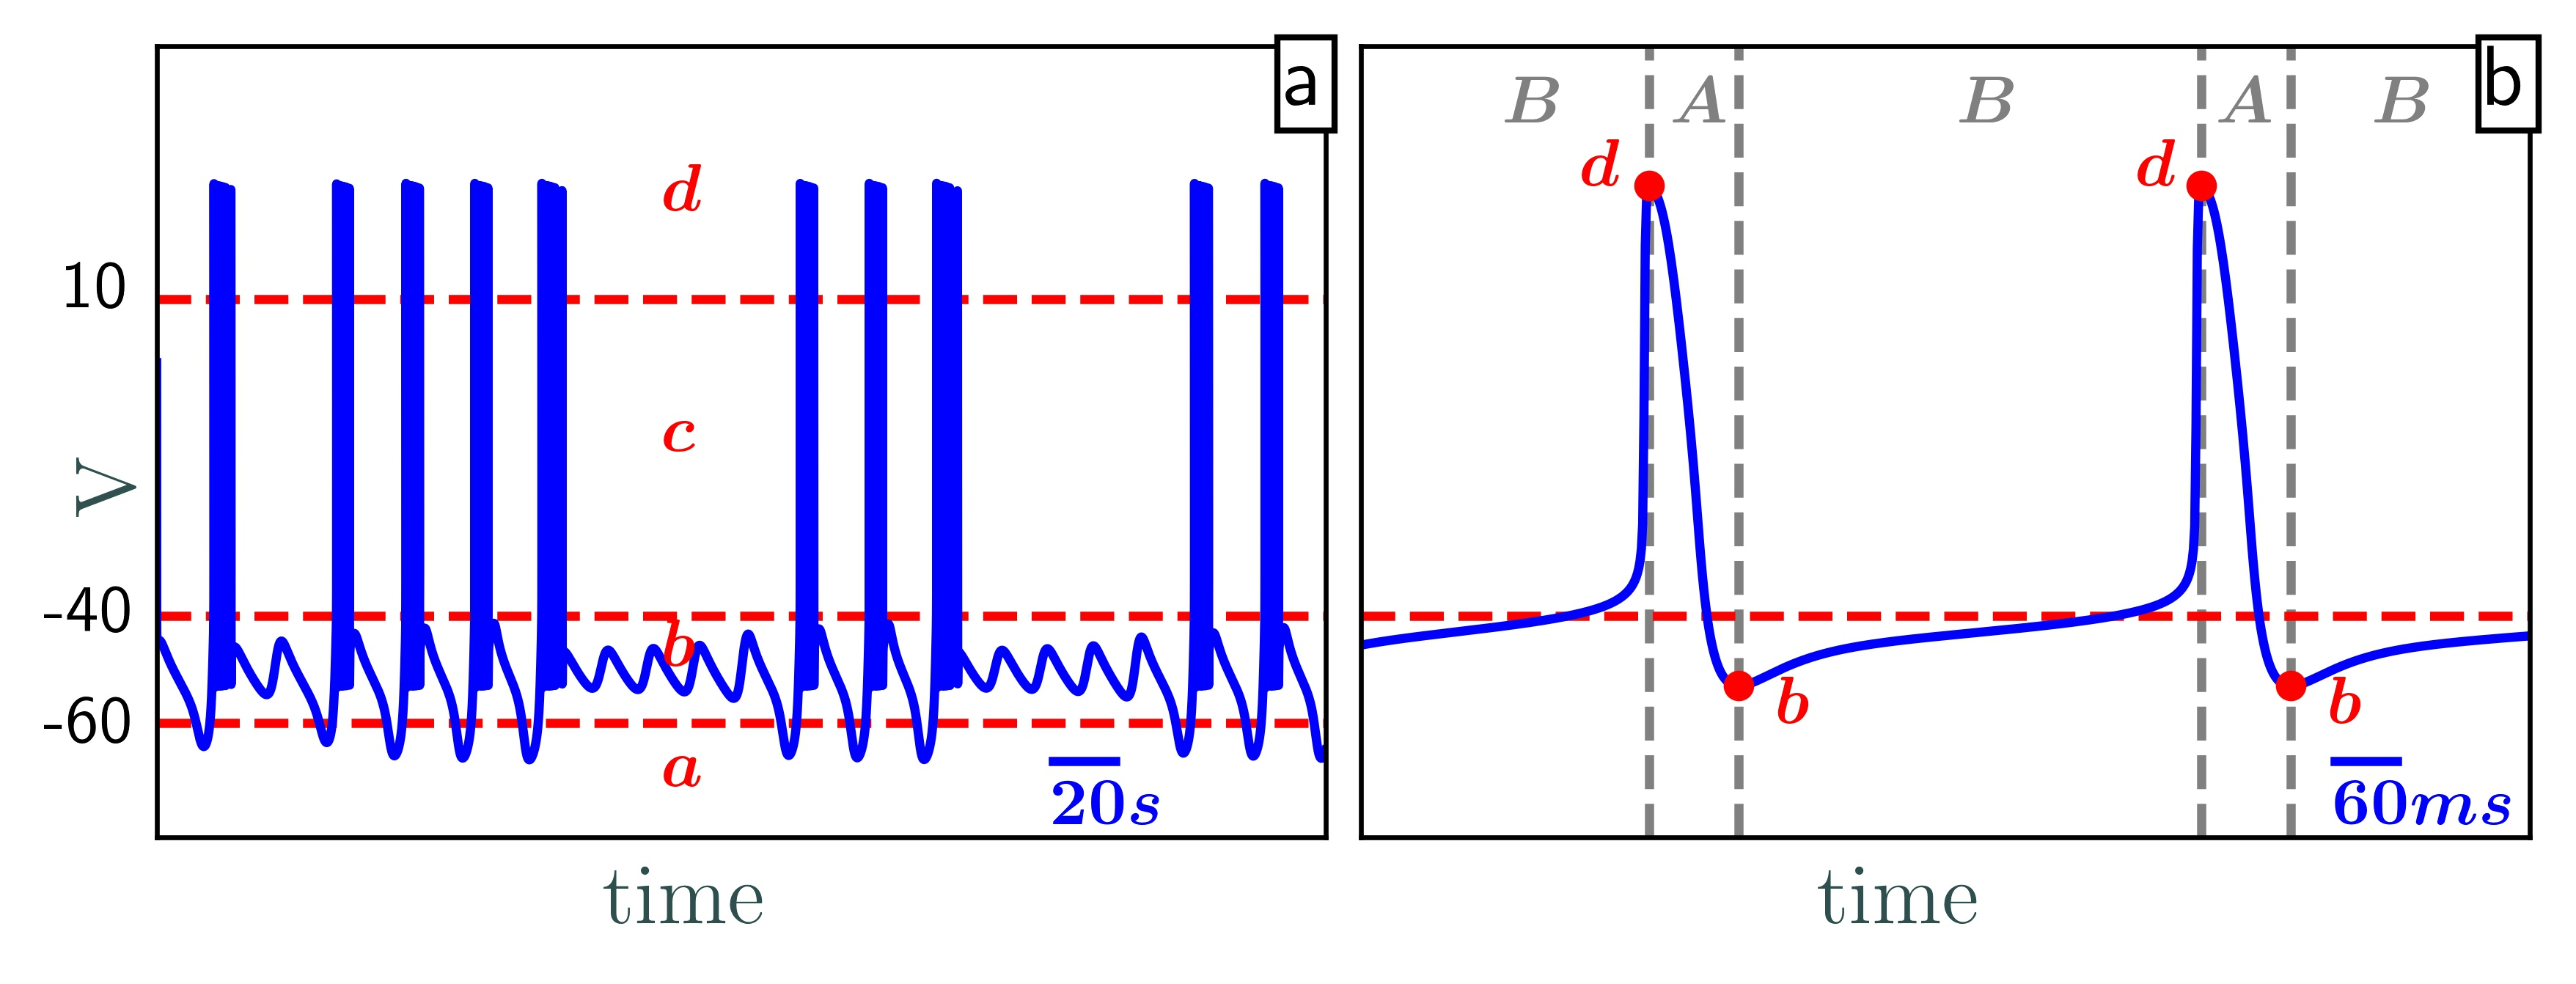
\includegraphics[width=1.03\textwidth]{DCPImages/Image0}
\caption{(a) Symbolic partitions demonstrated for mixed-mode chaotic bursting, partitioned by voltage levels at  $[-60, -40, 10]$mV (red dashed lines), resulting in a set of $4$ symbols $(a \leq -60 < b \leq -40 < c \leq 10 < d)$. A short segment showing two spikes in a burst is magnified in (b). Based on the occurrence of events of maximal and minimal voltage values (red dots) and using voltage partitions, the symbolic representation of this segment is coded as {\it (dbdb)} (in the red color). With time interval partitions $[100]$ms between events (gray dashed lines enclosing spikes) resulting in a set of 2 symbols $(A \leq 100 < B)$, the symbolic representation is given by $(BABAB)$ (in the gray color).  Combining both voltage and interval partitions gives a detailed symbolic sequence $(BdAbBdAbB)$.}\label{fig:plantTrajectory}
\end{figure}

In our previous studies implementing such a GPU-based (multi-core graphics processing unit)  symbolic toolkit, called Deterministic Chaos Prospector (DCP), we examined several  Lorenz-like systems \citep{pusuluri2017, pusuluri2018} to disclose a wealth of universal homoclinic and heteroclinic bifurcations of saddle equilibria, as well as to detect regions of simple and chaotic dynamics in the parameter space. Particularly, we relied on the $Z_2$-symmetry of such systems to generate and associate periodic or aperiodic binary sequences, corresponding to regular or chaotic flip-flop patterns of the  outgoing separatrix of the saddle at the origin. Unlike the case of the Lorenz-like attractors, chaos in slow-fast models of individual neurons is less typical. It generally occurs at transitions between bursting and tonic-spiking activity, when the corresponding orbit in the phase space changes its characteristics or stability through non-local bifurcations such as spike-adding, for example, through well-defined homoclinic bifurcations of periodic orbits and equilibria. The further development and use of the toolkit must, therefore, be motivated by a neuroscience-specific context based on the voltage wave-forms, without relying on having access to all the phase variables of a Hodgkin-Huxley model in question, such as the gating variables.     

One simple method for constructing a meaningful partition to differentiate between various voltage wave-forms is to break any given one into small time-bins of an identical size, shorter than the duration of a typical spike. As these bins sample over the trace, the occurrence of a spike within a bin is marked with the symbol $1$, and otherwise with $0$, thus digitizing the voltage trace into a binary sequence. Alternatively, we can identify events corresponding to maximal and minimal voltage values on all spikes in the trace. Whenever a maximum is detected in the trace above some {\em firing} threshold, we mark it with the symbol $1$, and whenever a minimum is detected below this threshold, we mark it with $0$. For a typical square-wave bursting trace (without sub-threshold oscillations), this approach would be identical to spike counting.  To stably identify a diverse set of neuronal dynamics including quiescent states, periodic tonic spiking, spike addition, square-wave bursting, plateau-busting, parabolic bursting, mixed-mode oscillations, quasi-periodicity and chaos, one should combine both voltage- and time-bin approaches, resulting in a minimal information loss algorithm that basically retains all relevant details, and describes the trace in the form of a multi-symbol string. 

Figure \ref{fig:plantTrajectory} illustrates one of the complex bursting traces with an unpredictable number of spikes within bursts that are separated by slow amplitude sub-threshold oscillations, also chaotic. Such a trace is typically recorded in the Plant endogenous parabolic burster \cite{deniz2015} at the transition between bursting activity and the hyper-polarized quiescent state. To find a symbolic description of this chaotic voltage trace, we first identify all events corresponding to maximal and minimal voltage values (red dots), as well as time intervals between them (gray dashed lines). We then use voltage and time interval partitions, $V_{bins}$ and $T_{bins}$, to symbolically characterize the event and timing information. Using the voltage partition $V_{bins} = [-60, -40, 10]$mV (red dashed lines) results in four symbols $(a \leq -60 < b \leq -40 < c \leq 10 < d)$, representing quiescence or burst terminations, sub-threshold oscillations, plateau burst, and spiking, respectively, found in a voltage trace. Similarly, the time interval partition $T_{bins} = [100]$ms results in a set of $2$ symbols, $(A \leq 100 < B)$, representing successive maximal/minimal events separated by a duration shorter or longer than $100$ms, respectively. Figure~\ref{fig:plantTrajectory}b shows a short segment of two spikes in a burst within the long voltage trace. The symbolic representations of this segment using $V_{bins}$, $T_{bins}$, and a combination of both, are given by $(dbdb)$ (red), $(BABAB)$ (gray) or  $(BdAbBdAbB)$, respectively. 

An overbar, like in $(\overline{abc})$, is meant to represent the periodic portion of a repetitive sequence that corresponds to regular tonic-spiking or bursting traces. For example, a tonic-spiking trace with two spikes like in Fig.\ref{fig:plantTrajectory}b might be represented by $(\overline{db})$, $(\overline{BA})$ or $(\overline{BdAb})$, respectively, with $V_{bins}$, $T_{bins}$ or combined partitions. Using just $V_{bins}$, spike addition to a burst starting from single spikes up to a burst with 4 spikes can be represented by $(\overline{da})$, $(\overline{dbda})$, $(\overline{dbdbda})$ and $(\overline{dbdbdbda})$, respectively. A quiescent state lacking all critical events is marked with the symbol $a$.

Omitting some long transient lets us examine long-term behaviors of solutions of the model in question. We normalize all shift-symmetric periodic sequences by designing a one-way hash function that produces identical hash value for all circular variations of a periodic sequence \citep{perlman2016}. In simple terms, all four circular variations of the periodic sequence $(\overline{abcd})$, $(\overline{bcda})$, $(\overline{cdab})$, or $(\overline{dabc})$ result in the same numerical hash value. For aperiodic strings representing chaotic traces, we use the LZ compression algorithm implemented in \cite{pusuluri2018} for deterministic chaotic systems, to measure its complexity. As the string is scanned, new words are continuously added to the vocabulary. Eventually, the size of the LZ-vocabulary normalized by the length of the string is used as the complexity measure.

\begin{figure}[ht!]
%\hspace{-22pt}
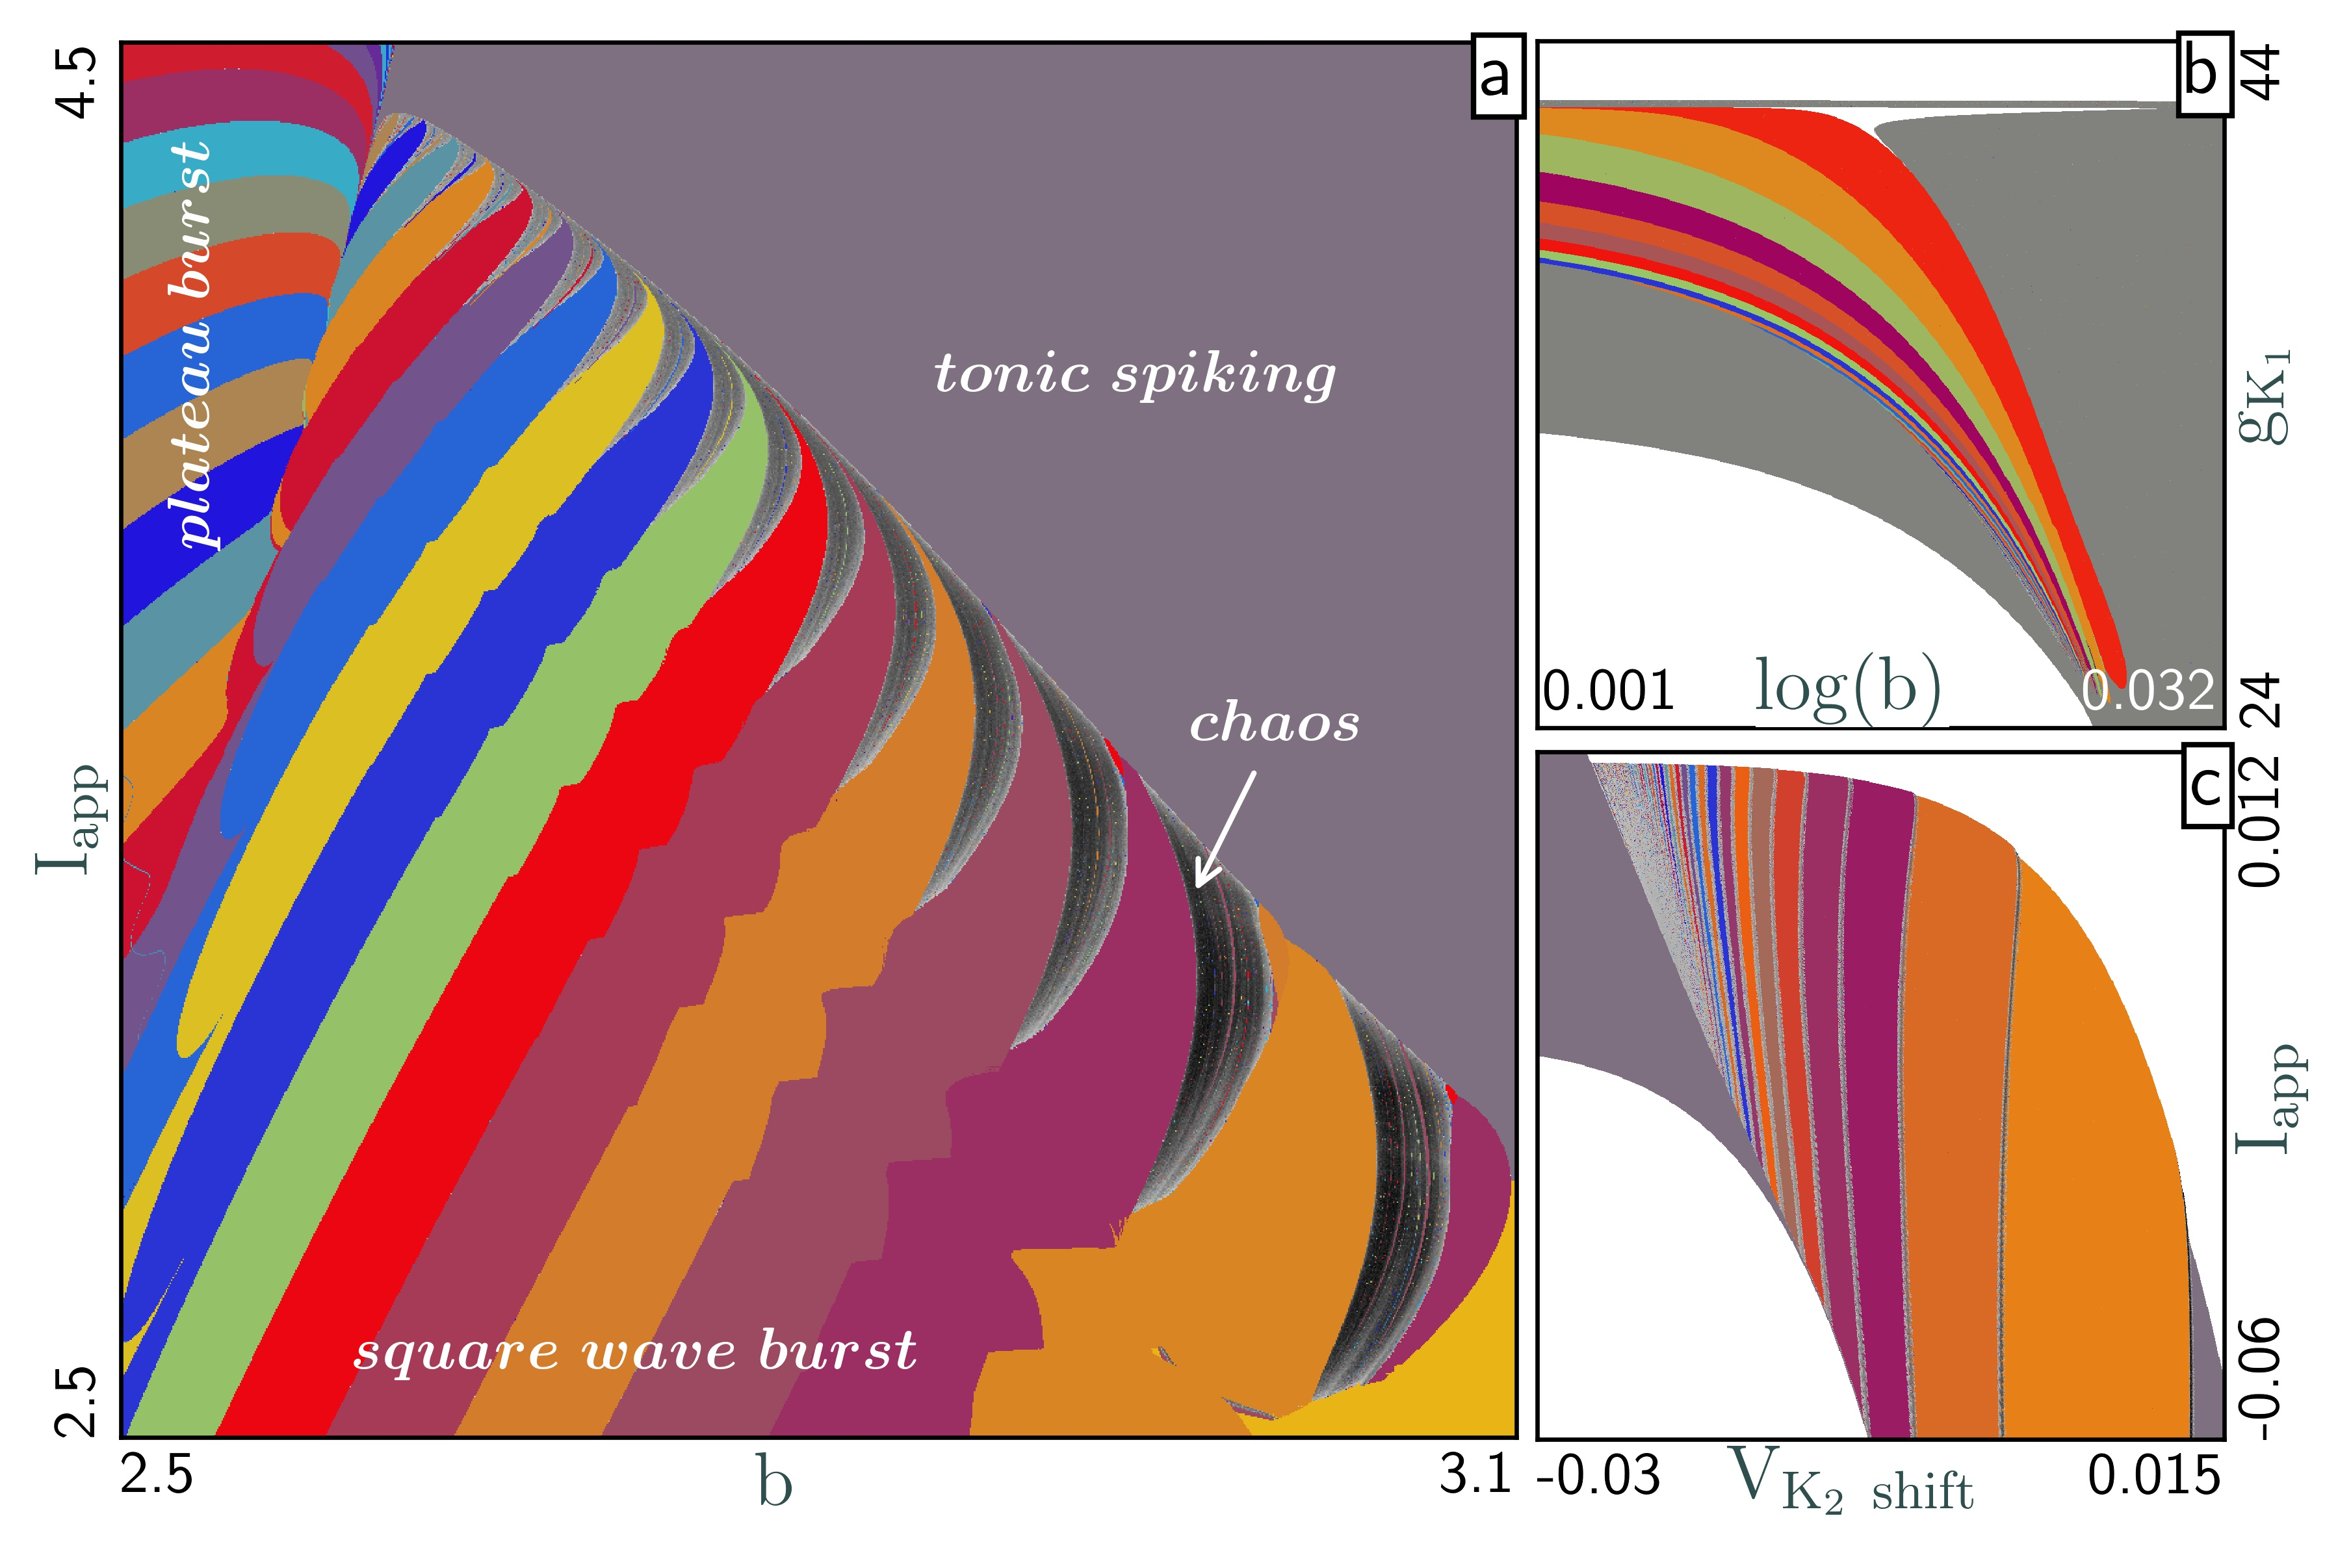
\includegraphics[width=1.\textwidth]{DCPImages/Image2}
\caption{Bi-parametric sweeps for the Hindmarsh-Rose model (a), the bull-frog hair cell model (b), and the leech interneuron model (c) using DCP reveal universal and diverse features. The HR model (a) demonstrates plateau-bursting and square-wave bursting in addition to tonic spiking (purple) and chaos (darker shades of gray imply greater LZ complexity). The bifurcation diagram is identical with $V$-bins $[-1.2]$ or $\tau$-bins $[25]$. Staircase-like patterns in (a) at the boundaries of spike adding transitions within the region of square-wave bursting are indicative of multi-stability. The hair cell model (b) shows tonic spiking (olive), quiescence (white), or bursting regions with spike-adding transitions between solid color stripes, same as in the bifurcation diagram of the leech interneuron model (c). Addition of noise in (c) widens the regions of chaos at the boundaries of spike addition.
}\label{fig:othermodels}
\end{figure}

\section{Bi-parametric sweeps}
Next, we demonstrate the benefits of this toolkit through highly detailed reconstructions of biparametric sweeps, shown in Fig.\ref{fig:othermodels}, for three neuronal models:  (a) a mathematical three-dimensional (3D) Hindmarsh-Rose model of a square-wave burster, (b) a highly detailed 12D bull-frog hair cell model featuring quasi-periodic oscillations, and another (c) 3D leech heart interneuron model featuring various bi-stable states and the blue-sky catastrophe bifurcation on the border of tonic-spiking and bursting activity; see Refs.~\citep{bar2011, barrio2014, neiman2011, ju2018, shilnikov2012} and the references therein, for details of the models and parameters. The biparametric sweeps are obtained by computing long traces using identical initial conditions as the two parameters are varied across a grid of size $1000\times 1000$. Numerical integration is performed using the fourth order Runge-Kutta method with fixed step size. The computation of these solutions is massively parallelized by running on separate GPU threads using CUDA, which results in fast computation of the sweeps such as Figure~\ref{fig:othermodels}a in about 200s. Visualizations are done in Python. A combination of $V_{bins}$ and $T_{bins}$ is employed to obtain symbolic sequences for events corresponding to the maximal and minimal voltage values, and/or time intervals. To study long-range dynamics of solutions of the models, a sequence of the first $2000$ symbols is omitted as transient. The following sequence of $2000$ symbols is then analyzed to detect the existence of periodicity (or lack thereof). If detected, the hash function generates the shift symmetric hash value of the periodic sequence, which is projected to a color map to obtain a color value. Parameter values that result in topologically identical periodic behavior in their solutions result in identical hash values, and thus, have identical color in the sweep. Aperiodic sequences are processed through the LZ-algorithm to detect their complexity. Lack of periodicity is indicative of structurally unstable, chaotic dynamics. They are represented in the bi-parametric sweeps in gray shades, with greater LZ-complexity shown in darker gray to represent greater instability. 

The bi-parametric sweeps shown in Fig.~\ref{fig:othermodels}  reveal a rich variety of dynamics in three typical neuronal models. Figure~\ref{fig:othermodels}(a) being a sweep of the Hindmarsh-Rose model, demonstrates regions of the plateau-  and square-wave bursting in addition to tonic spiking (purple) and chaos (gray shades). The bifurcation diagram remains identical with either $V_{bins} = [-1.2]$ or $\tau_{bins} = [25]$. At the boundaries of spike-adding bifurcations, one can spot a staircase-like pattern due to bi-stability of coexisting bursting solutions with distinct spike numbers, whose emergence depends on the choice of initial conditions.
Figure~\ref{fig:othermodels}(b) shows regions of tonic-spiking (olive), quiescence (white), or bursting with spike adding transitions between solid-color stripes in the bull-frog hair cell model. The boundary of the quiescent region (white) is due to the Andronov-Hopf bifurcations, while the boundary between tonic-spiking (olive) and bursting regions is due to torus and period-doubling bifurcations \citep{ju2018}. 
The leech interneuron model is also known to have regions of quiescence (white), tonic-spiking (purple) and bursting partitioned by spike-adding transitions within (other solid colors). Adding small noise to this model amplifies chaos at spike-adding bifurcations and widens its boundaries. \cite{channell2009}.  

\section{Conclusions and future directions}
We showed how a novel design of multi-bin voltage and time interval partitions enhancing the previously developed DCP-toolkit expedites examinations of dynamics of simple and biologically plausible models of individual neurons, and the sweeps of their parameter spaces, to a few seconds. It also provides the flexibility of minimal loss of voltage and timing information.  While this study employs manually built partitioning schemes, future development of the algorithms could apply statistical post-processing of event data to achieve scale-invariance and to enrich the high-resolution sweeps with additional temporal information concerning bursting and tonic-spiking activity. We also plan to extend these techniques for studies of the dynamics of neural networks. 

\section*{Acknowledgements}
This work was in part funded by NSF grant IOS-1455527, RSF grant 14-41-00044 at the Lobachevsky University of Nizhny Novgorod, and MESRF project 14.740.11.0919. We are grateful to Georgia State University`s Brains and Behavior initiative for fellowship and pilot grant support and to NVIDIA Corporation for the donation of Tesla K40 GPU used in this study. We thank all the members of Shilnikov NeurDS lab for helpful discussions.

%\input appendix.tex

% for BibTeX users
%\bibliographystyle{ws-book-har}    % Bibliography: Author-Date system
%\bibliography{ws-book-sample}      % pls. call your database here
%\bibliography{refsDCP}

% for non-BibTeX users
% \input bibliography.tex

\begin{thebibliography}{6}
\newcommand{\enquote}[1]{#1}
\providecommand{\natexlab}[1]{#1}
\providecommand{\url}[1]{\texttt{#1}}
\providecommand{\urlprefix}{URL }
\providecommand{\eprint}{eprint }
\expandafter\ifx\csname urlstyle\endcsname\relax
  \providecommand{\doi}[1]{doi:\discretionary{}{}{}#1}\else
  \providecommand{\doi}{doi:\discretionary{}{}{}\begingroup
  \urlstyle{rm}\Url}\fi


\bibitem{pusuluri2017}
K.~Pusuluri, A.~Pikovsky and A.~Shilnikov, \enquote{Unraveling the chaos-land
  and its organization in the Rabinovich system,} in \emph{Advances in
  Dynamics, Patterns, Cognition}.
\newblock Springer, 41 (2017).

\bibitem{pusuluri2018}
K.~Pusuluri and A.~L. Shilnikov, \enquote{Homoclinic chaos and its organization
  in a nonlinear optics model,}  \emph{Physics Review E} (2018), in press  \emph{arXiv:1806.01309}  

\bibitem{deniz2015}  
D.~Alacam and AL.~Shilnikov,  \enquote{Making a swim central pattern generator out of latent parabolic bursters,} \emph{Bifurcations and Chaos} \textbf{25}(7), 1540003 (2015).

\bibitem{perlman2016}
R.~Perlman, C.~Kaufman and M.~Speciner, \emph{Network security: private
  communication in a public world}.
\newblock Pearson Education India (2016).

\bibitem{bar2011}
R.~Barrio and AL.~Shilnikov, \enquote{Parameter-sweeping techniques for temporal dynamics of neuronal systems: case study of Hindmarsh-Rose model,} \emph{J Mathematical Neuroscience} \textbf{1}(6), (2011)

\bibitem{barrio2014}
R.~Barrio, M.~Angeles~Mart{\'\i}nez, S.~Serrano and A.~Shilnikov,
  \enquote{Macro-and micro-chaotic structures in the hindmarsh-rose model of
  bursting neurons,} \emph{Chaos: An Interdisciplinary Journal of Nonlinear
  Science} \textbf{24}, 2, 023128 (2014).

\bibitem{neiman2011}
A.~Neiman, K.~Dierkes, B.~Lindner and AL.~Shilnikov,  \enquote{ Spontaneous voltage oscillations and response dynamics of a Hodgkin-Huxley type model of sensory hair cells,} {\emph J. Mathematical Neuroscience,} \textbf{1}, 11, (2011)

\bibitem{ju2018}
H.~Ju, A.~Neiman and A.~Shilnikov, \enquote{Bottom-up approach to torus
  bifurcation in neuron models,} \emph{J. Chaos} \textbf{29}, 106317
  (2018).

\bibitem{shilnikov2012}
A.~Shilnikov, \enquote{Complete dynamical analysis of a neuron model,}
  \emph{Nonlinear Dynamics} \textbf{68}(3), 305 (2012).

\bibitem{channell2009}
P.~Channell,  I.~Fuwape, A.~Neiman, and AL.~Shilnikov,  \enquote{ Variability of bursting patterns in a neuronal model in the presence of noise}, \emph{J. Computational Neuroscience,} \textbf{27}(3), 527-542 (2009). 





\end{thebibliography}
\printindex

\end{document} 